\section{Evaluation}
\label{sec:evaluation}

We stress tested Floodlight-CD using the \texttt{pingall} command provided by Mininet.
This command goes through the host list and attempts to ping every other host in the topology.
\texttt{Pingall} was chosen since it requires that a new rule be written to the switch for both the request and reply of the majority of pings.
The only time a new rule is not written is if the rule already exists from a previous ping, i.e. when \texttt{h2} is pinging \texttt{h1} while the flow rules from \texttt{h1} pinging \texttt{h2} is still resident in the switch's flow table.
All flow rules in our tests were set with a one second hard timeout (the shortest Floodlight allows) to necessitate the writing of as many rules as possible to the switches.
This places a large load on Floodlight-CD to validate each rule as well as keep an up to date view of the switches' flow tables.
Since the installation of each dynamic rule is triggered by a packet being forwarded to the controller, the packets themselves are also checked to prevent controller based rule evasion.
Therefore, for every ping, the forward rule, the reverse rule, the request packet, and the response packet must be checked per switch for the ping to succeed.

\begin{figure*}[ht!]
	\begin{center}
		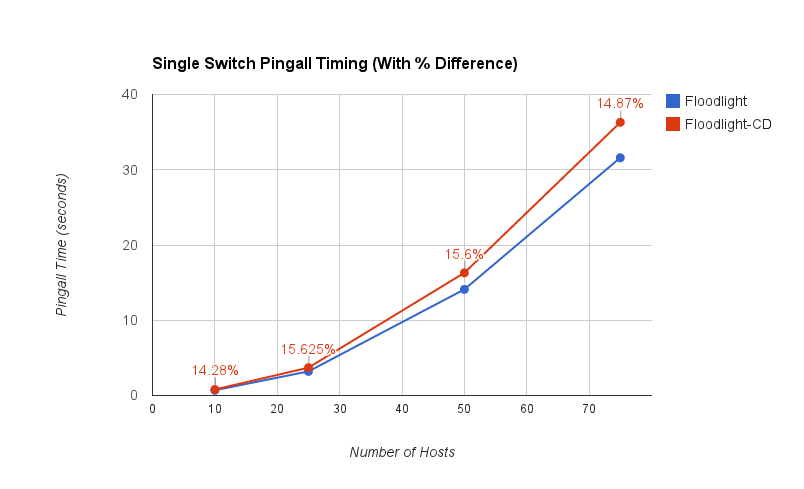
\includegraphics[scale=.5]{figs/singleSwitch_eval.png}
		\caption{Pingall timing with single switch and varying hosts}
		\label{fig:eval_single}
	\end{center}
\end{figure*}

The tests were done with varying numbers of switches and hosts.
Figure \ref{fig:eval_single} shows the performance of Floodlight-CD with a single switch and a varying number of hosts.
The addition of conflict detection results in a consistent overhead of about 15\%, regardless of the number of hosts.

\begin{figure*}[ht!]
	\begin{center}
		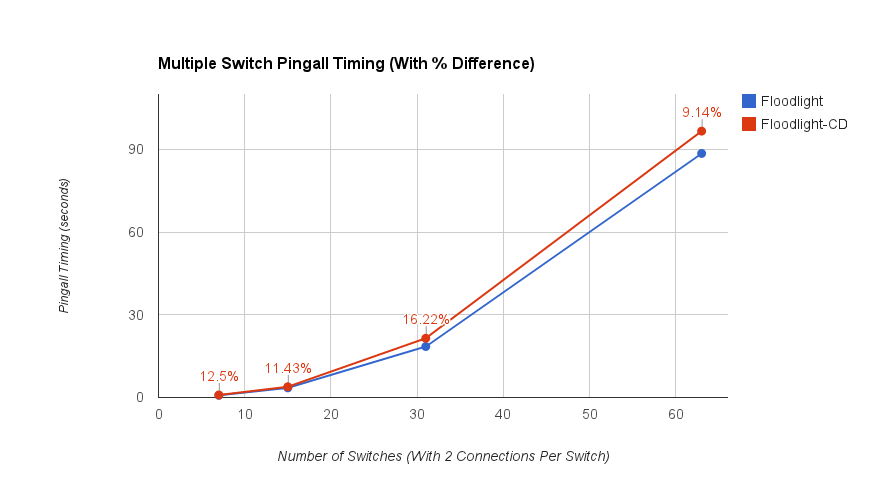
\includegraphics[scale=.5]{figs/multiSwitch_eval.png}
		\caption{Pingall timing with varying switches}
		\label{fig:eval_multi}
	\end{center}
\end{figure*}

Figure \ref{fig:eval_multi} shows the timing data for topologies with multiple switches.
All of these tests were run using the tree topology where the number of levels of the tree were varied.
Each leaf switch had two hosts connected to it.
We found these tests to truly exercise Floodlight-CD due to the number of switches involved in a single ping between hosts on opposite sides of the tree.
When a host pings a destination on the other side of the tree, the forward and reverse rules must be checked and installed on (2*L) - 1 switches, where L is the number of levels of the tree. 
The overhead incurred by conflict detection in a multi-switch scenario varied from 9\% up to 16\%, with an overall average being about 15\%.

While an average overhead of 15\% for all scenarios is not terrible, we believe that this could be reduced.
We spent a large amount of time working through concurrency issues within Java.
We believe that our implementation can be optimized to increase the performance of Floodlight-CD.

